% Artigo unico do ADR 0006 (MSSP). Rascunho de 2026-11-13, revisado contra a revisao adversarial do
% manuscrito inteiro (reviewer-2, mesmo dia): pre-registro por experimento, livro-razao das hipoteses
% no apendice, manchete do Paderborn com IC e especificidades. Faltam autores, link do codigo,
% declaracoes da Elsevier e compilacao. Referencias so do literature/refs.bib (campo verified).
\documentclass[preprint,12pt,authoryear]{elsarticle}
\usepackage{amsmath,amssymb}
\usepackage{graphicx}
\usepackage{booktabs}
\usepackage{longtable}
\usepackage{siunitx}
\usepackage[colorinlistoftodos]{todonotes}
\usepackage{hyperref}

\journal{Mechanical Systems and Signal Processing}

\begin{document}

\begin{frontmatter}

\title{Blind band selection under pure decimation of bearing vibration: aliased impulses,
fault-order decisions and a power check for learned sampling}

\author{\todo[inline]{Author list and affiliations: decided by the student and the advisor.}}

\begin{abstract}
A node that lowers its sampling rate behind a front end fixed for the highest rate cannot band-pass
filter an unknown fault resonance. Pure decimation is the limiting case: everything outside the band
folds with it. We study how the folded content affects blind band selection in three bearing
benchmarks. On Ottawa, a quasi-periodic train of single-sample spikes, present in every record
including healthy ones, captures the kurtogram on outer-race records from $3\times$ to $6\times$,
and order-estimation accuracy falls non-monotonically with the factor. An anti-alias filter at the
reduced rate avoids the capture at no cost, and three steps that need no full-rate access do the
same at $4\times$. Injected bursts reproduce the capture on CWRU, while a phase-randomized surrogate
with the same folded spectrum does not. On Paderborn, where the kurtogram is captured at full rate,
a decision restricted to the fault orders of the bearing geometry, with a threshold from six
healthy bearings, identified the faulty race in 49--51\% of segments at $4\times$ and $8\times$,
against 16--19\% for blind order estimation (+33 points, 95\% interval +16 to +50), at 94\% against
100\% specificity. The advantage was as large at full rate, and an anti-alias filter beat pure
decimation by 7 to 30 points. A power gate showed that our pre-registered test could not detect even
a perfect learned method on Ottawa, unlike on Paderborn. Learned sampling masks did not outperform
trained uniform decimation or random masks, but the intervals do not exclude a gain of 5 points.
\end{abstract}

\begin{keyword}
bandpass sampling \sep aliasing \sep spectral kurtosis \sep kurtogram \sep impulsive noise
\sep learned sampling \sep rolling element bearings
\end{keyword}

\end{frontmatter}

\listoftodos

\section{Introduction}
\label{sec:intro}

The diagnostic content of rolling-element bearing vibration sits far above its modulation rate.
A localized defect excites structural resonances, and the fault frequency only appears as the
repetition rate of the excited transients. In the Paderborn benchmark
\citep{lessmeier2016paderborn}, the resonance that carries an electrical-discharge outer-race
defect occupies roughly 2.5--4.4~kHz, and the one that carries inner-race defects 8.4--11~kHz,
while the fault orders are 3.05 and 4.95, that is, about 76~Hz and 124~Hz at 1500~rpm
(Section~\ref{sec:data}). Sampling such signals at twice their highest frequency is costly in
energy and in data, and it is not what the information requires.

The rate that the information requires is set by the occupied bandwidth, not by the highest
frequency. This is the content of Landau's theorem \citep{landau1967}: the minimal average
sampling density of a signal is the measure of its spectral support. Bandpass sampling realizes
it for a single band with uniform sampling at suitable rates \citep{vaughan1991}, and multicoset
sampling realizes it for unions of bands at any position
\citep{venkataramani2001optimal,mishali2009xampling}. Operating below the Nyquist rate is therefore
not a departure from sampling theory; it is the regime that sampling theory prescribes for
structured signals. Envelope analysis of bandpass-sampled vibration has been shown to keep bearing
fault signatures well below the Nyquist rate \citep{lu2018undersampled}.

Blind envelope analysis, however, needs a band selector, and the standard one is spectral kurtosis
through the fast kurtogram \citep{antoni2007kurtogram}. Spectral kurtosis measures impulsiveness,
not periodicity, and it is known to be captured by impulsive interference that is not related to
the fault: electromagnetic interference from variable-frequency drives \citep{smith2016emi,
vaerenberg2025cyclicemi} and non-cyclic impulsive noise in general
\citep{hebdasobkowicz2020nongaussian,hebdasobkowicz2025robustcorr}. All of these studies assume a
conventional acquisition, with an anti-alias filter in front of the converter. In that setting the
filter confines the interference to the acquisition band; \citet{vaerenberg2025cyclicemi} even
note that the anti-alias filter acts as the carrier band of the EMI impulses.

Pure decimation below the Nyquist rate removes that filter by design, because bandpass sampling
needs the resonance band to fold into baseband. Whatever impulsive content lies outside the band
of interest folds as well, and it may land on the range that the selector searches. Whether, when
and how strongly this happens has not been studied, as far as our searches show: keyword searches
and forward-citation tracking of \citet{smith2016emi} and \citet{vaerenberg2025cyclicemi} found no
work on band selection under decimation or folding (Section~\ref{sec:related}).

This paper studies that interaction and its consequence for learned acquisition.
\todo[inline]{Contributions: confirm each against the final results before submission.}
\begin{enumerate}
  \item We show, on the public Ottawa benchmark \citep{huang2018ottawa}, that single-sample spikes
  present in the raw records, healthy ones included, capture kurtogram band selection under pure
  decimation and produce a non-monotonic loss of order-estimation accuracy with the decimation
  factor. Removing the spikes before decimation restores the accuracy, in a pre-registered test.
  Three simple steps that need no access to the full-rate record do the same at $4\times$:
  cleaning isolated outliers in the decimated stream, a three-point median, and a lower search
  ceiling. Each has a limit, which we report.
  \item We reproduce the capture causally by injecting impulsive interference into the CWRU
  benchmark \citep{smith2015cwru}, against a phase-randomized surrogate with the same spectrum.
  \item We test the same interventions on the Paderborn benchmark, whose drive is fed by a 16~kHz
  PWM inverter. There, the kurtogram is already captured at full rate, decimation produces no
  valley, spike removal changes little, and the SES infogram \citep{antoni2016infogram} helps only
  at the lowest rate. A lower search ceiling at full rate gains more than decimation, though short
  of significance in a pre-registered test. The replication shows when the mechanism's
  precondition, a selector that is right at full rate, is absent.
  \item We show with a pre-registered power gate that a widely used benchmark cannot detect any
  improvement over a training-selected uniform rate, not even from a perfect estimator, while
  another can. We argue that such a gate should precede the training of learned acquisition on
  condition-monitoring data.
  \item We test learned sampling masks under a hardware-feasible set on both benchmarks, at equal
  or lower average rate. The learned mask does not outperform uniform decimation trained on the
  same records or a random mask at any budget from 1/4 to 1/32. On Paderborn, where a gain of 5
  points was detectable, the differences stay within $-5.2$ and $+4.4$ points, and the margin over
  the classical pipeline belongs to the decoder that all masks share.
\end{enumerate}

\section{Related work}
\label{sec:related}

\paragraph{Sampling below the Nyquist rate}
Landau's density theorem gives the minimal average rate for signals with a known spectral support
\citep{landau1967}. For a single band, uniform bandpass sampling reaches it at rates that place the
band within one Nyquist zone \citep{vaughan1991}. Multicoset sampling reaches it for unions of bands
in arbitrary positions \citep{venkataramani2001optimal}, and the modulated wideband converter and
the Xampling framework extend it to unknown supports \citep{mishali2009xampling,mishali2010practice,
eldar2015}. In all of these, aliasing is not an artefact to be avoided but the mechanism that makes
the rate reduction possible. Noise present in the signal before subsampling folds with it and is
amplified by the subsampling factor, the noise folding of compressed sensing
\citep{ariascastro2011noisefolding}. What folds along with the band of interest, and what it does
to a blind band selector, is the subject of this paper.

\paragraph{Band selection for bearing diagnostics under impulsive interference}
The fast kurtogram selects the demodulation band by spectral kurtosis \citep{antoni2007kurtogram}.
Its sensitivity to impulsive noise motivated the infogram, which measures the negentropy of the
squared envelope and of its spectrum; the latter responds to repetitive transients and is
insensitive to isolated impulses \citep{antoni2016infogram}. \citet{smith2016emi} showed that
inverter EMI defeats spectral-kurtosis band selection and proposed restricting the bandwidth.
\citet{vaerenberg2025cyclicemi} removed periodic EMI with cyclic Wiener (FRESH) filters before a
higher-resolution kurtogram. \citet{hebdasobkowicz2020nongaussian} compared seven selectors under
cyclic and non-cyclic impulses and found that, with large non-cyclic impulses, only a selector based
on conditional variance identified the cyclic band \citep{hebdasobkowicz2020condvar}; robust
correlation maps were proposed for heavy-tailed signals \citep{hebdasobkowicz2025robustcorr}. These
works establish that non-fault impulses capture blind selectors at full rate, with an anti-alias
filter in place. None considers decimation.

\paragraph{Bearing diagnostics below the Nyquist rate}
Bandpass sampling followed by envelope analysis keeps bearing signatures at rates well below the
Nyquist rate \citep{lu2018undersampled}. Multirate and adaptive schemes have been proposed
\citep{elbouharrouti2023multirate,zhao2026adaptive}, as have compressive approaches with random
sampling \citep{ahmed2018compressedbearing,tounsi2026cs}. These studies evaluate diagnostic
accuracy under reduced sampling. None of them, to our knowledge, examines where a blind band
selector goes when interference folds.

\paragraph{Learned acquisition}
In magnetic resonance imaging, sampling masks are learned jointly with the reconstruction
\citep{bahadir2020loupe,huijben2020dps}, under physical trajectory constraints
\citep{weiss2021pilot}, and adaptively per measurement \citep{vangorp2021adps}. At moderate
acceleration, learned policies have been found on par with handcrafted equidistant masks, and the
best ones learned to be non-adaptive \citep{bakker2022adaptive}. Task-based acquisition learns the
converter for the downstream task \citep{shlezinger2022taskadc}, and its power-aware version learns
the quantization regions of a memristive converter \citep{vol2024poweraware}, that is, the bits
rather than the sampling times. Algorithm unrolling gives interpretable decoders built from the
classical pipeline \citep{monga2021unrolling}.

\section{Data and methods}
\label{sec:methods}

Every hypothesis, decision rule and test below was written and committed before the corresponding
run; the commit history of the repository records the order. Values given here are those of the
experiment configurations.
\todo[inline]{Cite the code and data release (repository link) before submission.}

\subsection{Datasets}
\label{sec:data}

\paragraph{Ottawa}
The University of Ottawa benchmark \citep{huang2018ottawa} records bearing vibration under
time-varying speed at 200~kS/s, with an accelerometer and a shaft encoder; we count 1024 encoder
pulses per revolution, a value inferred from the data because it is not documented. It contains
healthy, inner-race and outer-race conditions under four speed scenarios, with three trials each.
The bearing has nine rolling elements and a diameter ratio $d/D = 0.2067$, so the fault orders are
$\mathrm{BPFO} = 3.570$ and $\mathrm{BPFI} = 5.430$. Records are cut into 2.5~s segments.

\paragraph{CWRU}
The drive-end 48~kS/s records of the Case Western Reserve University benchmark, with the
categorization of \citet{smith2015cwru}, host the injected-interference experiment.

\paragraph{Paderborn}
The Paderborn benchmark \citep{lessmeier2016paderborn} records 6203 bearings at 64~kS/s in a drive
fed by a PWM inverter with 16~kHz switching. We use the three settings at 1500~rpm, whose 4~s
measurements resolve 0.010 order, and the 23 bearings with single-race damage: 12 outer-race (7
artificial, 5 from accelerated lifetime tests) and 11 inner-race (5 artificial, 6 real). The
geometry of the FAG bearing (8 balls, $d = 6.75$~mm, $D = 28.55$~mm, contact angle $0^\circ$) gives
$\mathrm{BPFO} = 3.054$ and $\mathrm{BPFI} = 4.946$ orders; the manufacturers used vary by up to
1--2\% in characteristic frequencies \citep{lessmeier2016paderborn}.

The 64~kS/s record length varies between files while the stored time axis always spans 4~s. We
checked the time base with the motor current: the drive is a synchronous machine with four pole
pairs, so its electrical frequency is exactly four times the shaft speed, which is recorded on a
separate 4~kHz channel. With a fixed 64~kS/s, the ratio between the two has a median of 0.99998
over 2559 readable files, and only one file deviates by more than 0.5\%; the alternative reading,
in which the stored time axis is correct, puts 185 files beyond 0.5\%. We therefore use 64~kS/s
throughout, cut every measurement to 255\,936 samples (4~s minus 1~ms) aligned with the speed
channel, and exclude shorter or unreadable measurements.

\subsection{Acquisition model}

Sub-Nyquist acquisition is modelled by pure decimation, $x_M[n] = x[nM]$, of the full-rate record,
which is an ideal sampler at $f_s/M$ with no anti-alias filter. No track-and-hold bandwidth,
aperture jitter or quantization is modelled; the cost metric is the number of converted samples
per second. Because the records were acquired with the anti-alias filter of the original
instrument, content above the original Nyquist frequency is absent, and the folding studied here
is that of content between the effective and the original Nyquist frequencies.

\subsection{Classical pipeline}
\label{sec:pipeline}

The baseline is the classical envelope pipeline. The band is chosen by a fast kurtogram
\citep{antoni2007kurtogram} with ideal FFT band masks, dyadic and one-third-dyadic levels up to
level 4, and a search range from 500~Hz to a ceiling. The ceiling is 25~kHz for Ottawa, below
which lies more than 99.9\% of the record energy, and the effective Nyquist frequency for
Paderborn. The squared envelope of the
band is resampled in angle at 64 samples per revolution with an angular anti-alias filter, and the
order estimate is the maximum of the order spectrum above order 2, with no prior on the fault
order. A run is discarded, and counted as a miss, when the decimated record has fewer than 4096
samples, when the effective Nyquist frequency falls below the search floor, or when fewer than
$g \times 64$ samples per revolution remain, with $g = 2$ for Ottawa and $g = 1$ for Paderborn.

\subsection{Ground truth}
\label{sec:truth}

The fault order is known from geometry only up to slip and manufacturing spread, so the truth is
calibrated from the full-rate data, never from the arm under test.
\begin{itemize}
  \item \emph{Local ruler}: the order of the full-rate line in the same segment, refined around
  the geometric order by harmonic-energy score and taken at the centre of the score plateau. The
  search spans $\pm12\%$ for Ottawa and $\pm1\%$ for Paderborn. For Paderborn the line must also
  stand out: its peak must reach at least five times the median of the order spectrum within
  $\pm7\%$ of the geometric order. A segment without a valid line has no local truth.
  \item \emph{Nested ruler}: the median of the valid calibrations of other records of the same
  race, outside the test set. In E24, which has no training, the bearing under test is left out.
\end{itemize}
An estimate is a hit when it falls within 0.06 order of the truth for Ottawa and 0.025 order for
Paderborn. The tighter tolerance is forced by geometry: the Paderborn BPFO and BPFI lie 0.054 order
from the third and fifth shaft harmonics, and a looser tolerance would score a line locked on the
harmonic as a hit. Accuracy is balanced: the mean over races of the per-unit hit rate.

\subsection{Spike removal}

A sample is an isolated spike when its deviation from the mean of its two neighbours,
$\delta[n] = x[n] - \tfrac12(x[n-1] + x[n+1])$, exceeds ten times
$1.4826\,\mathrm{median}|\delta|$, and both neighbours deviate in the opposite direction by less
than 0.8 of it. Spikes are replaced by the mean of their neighbours. Applied at full rate, before
decimation, the procedure is not realizable on a decimating node; it is a diagnostic intervention
that attributes the loss to the spikes. A single-sample spike that survives decimation lands on a
kept sample and stays isolated in the decimated stream, so the same criterion can also be applied
after decimation, at the effective rate, where it is realizable. This variant is tested as a
separate arm.

\subsection{Attribution by folding zone}
\label{sec:zones}

At $4\times$ on Ottawa the effective Nyquist frequency is 25~kHz, equal to the search ceiling. The
upper half of the search range at the first kurtogram level, $[12.75, 25]$~kHz, then receives the
folded content of three zones of the original frequency axis: $Z_1 = [25, 37.25]$,
$Z_2 = [62.75, 75]$ and $Z_3 = [75, 87.25]$~kHz. To attribute the loss, each zone, and their
union, is rejected at full rate before decimation by an ideal zero-phase FFT mask. An ideal
anti-alias filter, which zeroes everything above the effective Nyquist frequency, and a
three-point running median complete the interventions. None of these masks is realizable; their
purpose is causal attribution.

\subsection{Robust band selectors}

Two selectors replace spectral kurtosis on the same band partition. The SES infogram
\citep{antoni2016infogram} computes, for each band, the energy flow $\varepsilon[n] = |c[n]|^2$ of
the analytic band signal sampled at its critical rate, and the negentropy of the squared-envelope
spectrum without its zero-frequency term,
\begin{equation}
  \Delta I_E = \left\langle \frac{|E(\alpha)|^2}{\langle |E|^2\rangle}
  \ln\frac{|E(\alpha)|^2}{\langle |E|^2\rangle} \right\rangle_{\alpha \neq 0},
\end{equation}
where $E$ is the discrete Fourier transform of $\varepsilon$. Our implementation reproduces the
values that \citet{antoni2016infogram} gives for stationary Gaussian noise (1.1525 for the
time-domain and 0.4228 for the spectral negentropy). The spectral Gini index
\citep{hebdasobkowicz2020nongaussian} replaces the kurtosis by the Gini index of the band envelope.

\subsection{Statistical protocol}
\label{sec:stats}

Accuracy differences are tested with a cluster bootstrap whose unit is the independent source of
variation. For Ottawa, that is the condition-by-scenario cluster, four per race. For Paderborn, it
is the bearing. Units are resampled with replacement within each race, together with the
cross-validation folds when there are any, and the one-sided p-value is
$(1 + \#\{\Delta^* \le 0\})/(1 + B)$ with $B = 4000$. A zero difference therefore counts against the
hypothesis. Holm's correction is applied within each family of tests. Paired segment-level
comparisons in the Ottawa intervention study use the exact McNemar test.

\paragraph{Power gate}
Before training any learned method, we asked whether a benchmark can detect an improvement at all.
A planted arm is derived from the baseline by turning each of its misses into a hit with
probability $q$, using the same draw for both rulers, with $q$ chosen for gains of +5 and +10
points or for a perfect arm. The pre-registered decision rule is then applied with all other
comparisons assumed significant, which is deliberately optimistic, so that a negative answer is
conclusive. A benchmark passes if the power at +5 points reaches 0.80 in some admissible design.

\subsection{Learned sampling masks}
\label{sec:masks}

For a budget of one sample in $b$, the feasible set allows $K = 4$ active ticks in each period of
$L = 4b$ ticks, with a minimum gap of two ticks between them. This is the class of periodic
nonuniform patterns that a timer-triggered converter can schedule. Masks are learned by a top-$K$
Gumbel relaxation with a straight-through estimator and an annealed temperature. The mask is
trained jointly with an unrolled decoder \citep{monga2021unrolling} that mirrors the classical
pipeline:
\begin{itemize}
  \item a learnable complex filter bank;
  \item the squared envelope;
  \item angular resampling;
  \item order-spectrum logits.
\end{itemize}
The decoder has no learned term per order bin, so it cannot place a peak where the data have none.
Early stopping and checkpoint selection start only after the annealing ends. A budget is evaluable
only if the masks left the Gumbel noise, that is, if the margin between the $K$-th and
$(K{+}1)$-th logits exceeds the noise standard deviation, in at least half of the splits.

The learned masks are compared with:
\begin{itemize}
  \item the best uniform rate at or below the budget, chosen on training data;
  \item the same decoder with that uniform mask;
  \item a fixed random feasible mask;
  \item multicoset designs, including that of \citet{venkataramani2001optimal};
  \item a mask learned without the constraint and projected onto it afterwards
  \citep{huijben2020dps,weiss2021pilot}.
\end{itemize}

On Paderborn, cross-validation is by bearing, in four folds stratified by race, with three seeds
per fold. Training labels come from the nested ruler, because the local ruler exists for only 6 of
the 23 bearings.

\section{Results}
\label{sec:results}

Each figure and table is regenerated from the \texttt{metrics.csv} of its experiment (scripts in
\texttt{papers/shared/figures}).

\subsection{The decimation valley on Ottawa and its captor}
\label{sec:res-valley}

Table~\ref{tab:ottawa} and Fig.~\ref{fig:valley} give the order hits of the outer race under pure
decimation, with the 25~kHz search ceiling.
\begin{itemize}
  \item At full rate the classical pipeline hits 27 of 36 segments under the nested ruler and 31 of
  35 under the local ruler.
  \item Decimation by 3 to 6 brings both down to 2--11 hits. The valley closes again at $8\times$,
  with 25 and 28 hits.
  \item The inner race is not affected: it stays at 35--36 of 36 hits in every cell, under both
  rulers.
\end{itemize}

The selected band shows where the loss comes from. At full rate the kurtogram selects a band
between 2.0 and 4.6~kHz in 32 of the 36 outer-race segments, and a band above 12.75~kHz in 2. At
$4\times$ the raw records move it to $[12.75, 25]$~kHz, the band that receives the three folding
zones of Section~\ref{sec:zones}, in 26 of 36 segments, and above 12.75~kHz in 29.

Removing the single-sample spikes before decimation closes the valley, and the selection at
$4\times$ returns to the band chosen at full rate (3 of 36 above 12.75~kHz).
\begin{itemize}
  \item At $4\times$ the pipeline hits 28 of 36 segments against 6, with all 22 discordant pairs in
  favour (exact McNemar, $p = 4.8\times10^{-7}$). Under the local ruler it hits 32 of 35
  ($p = 3\times10^{-8}$).
  \item Because the three segments of a record are not independent, the comparison was repeated
  at record level as a sensitivity analysis: 11 of the 12 outer-race records improve and none
  worsens (exact sign test, $p = 0.001$).
  \item The three-point median gives the same counts up to $4\times$, and the ideal anti-alias filter
  gives 27 hits at every factor up to $5\times$.
\end{itemize}

The zone rejections attribute the loss at $4\times$. Rejecting $Z_1$ alone leaves 7 hits against
6, rejecting $Z_2$ or $Z_3$ alone recovers 21, and rejecting the three recovers 27, the same as the
ideal anti-alias filter. Lowering the search ceiling to 12.5~kHz also avoids the valley: the
raw records then stay at 27--29 hits from $1\times$ to $6\times$.

\begin{table}[t]
  \centering
  \caption{Outer-race order hits on Ottawa under pure decimation, with the 25~kHz search ceiling
  unless stated. Each cell gives the hits under the nested ruler (of 36 segments) and, in
  parentheses, under the local ruler (of 35; one segment has no valid full-rate line). The zones
  are the original-frequency intervals that fold onto $[12.75, 25]$~kHz at $4\times$.}
  \label{tab:ottawa}
  \small
  % gerado por papers/shared/figures/tab_ottawa_valley.py a partir de
% experiments/E20-fold-zone-rejection/results/metrics.csv; nao editar a mao.
% celula: acertos na regua aninhada (de 36) e, entre parenteses, na local (de 35)
\begin{tabular}{lccccccc}
\toprule
 & \multicolumn{7}{c}{decimation factor $M$} \\
\cmidrule(lr){2-8}
intervention before decimation & 1$\times$ & 2$\times$ & 3$\times$ & 4$\times$ & 5$\times$ & 6$\times$ & 8$\times$ \\
\midrule
raw, no intervention & 27 (31) & 20 (22) & 4 (4) & 6 (6) & 2 (2) & 11 (11) & 25 (28) \\
reject $Z_1$ (25--37.25~kHz) & 27 (31) & 20 (22) & 4 (4) & 7 (7) & 3 (3) & 12 (12) & 25 (28) \\
reject $Z_2$ (62.75--75~kHz) & 27 (31) & 20 (22) & 4 (4) & 21 (24) & 12 (13) & 12 (12) & 26 (29) \\
reject $Z_3$ (75--87.25~kHz) & 27 (31) & 28 (32) & 19 (21) & 21 (24) & 2 (2) & 24 (27) & 26 (29) \\
reject $Z_1 \cup Z_2 \cup Z_3$ & 27 (31) & 28 (32) & 21 (23) & 27 (31) & 15 (16) & 23 (26) & 29 (32) \\
ideal anti-alias filter & 27 (31) & 27 (31) & 27 (31) & 27 (31) & 27 (29) & 25 (28) & 27 (30) \\
single-sample spikes removed & 28 (32) & 28 (32) & 28 (32) & 28 (32) & 27 (30) & 24 (27) & 29 (32) \\
3-point median & 28 (32) & 28 (32) & 28 (32) & 28 (32) & 25 (28) & 25 (28) & 28 (31) \\
\midrule
raw, search ceiling 12.5~kHz & 27 (30) & 28 (31) & 28 (31) & 29 (32) & 29 (32) & 29 (32) & 25 (28) \\
\bottomrule
\end{tabular}

\end{table}

\begin{figure}[t]
  \centering
  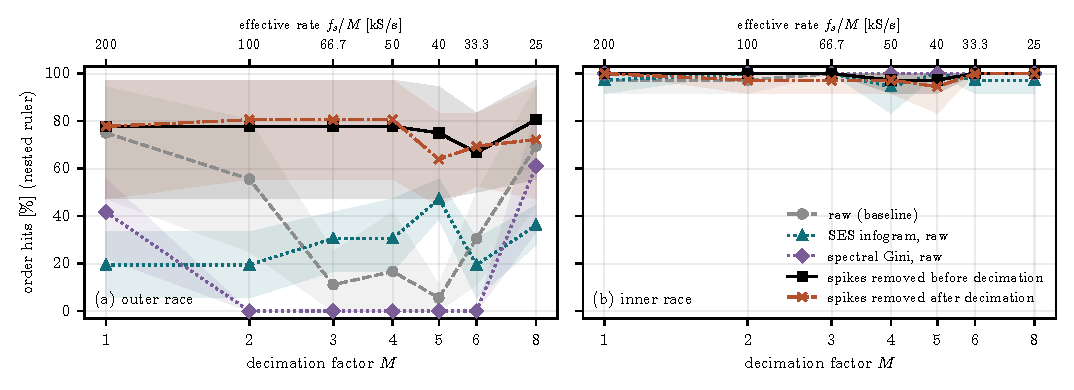
\includegraphics{figures/fig_valley_nested.pdf}
  \caption{Order hits against the decimation factor on Ottawa, under the nested ruler, for the
  outer race (a) and the inner race (b). The shaded bands are 95\% intervals from a bootstrap over
  the four condition-by-scenario clusters of each race; with four clusters they are wide. The top
  axis gives the effective rate.}
  \label{fig:valley}
\end{figure}

\subsection{Injected interference}
\label{sec:res-injected}

CWRU 48k has no native high-band interferer, and its classical baseline degrades monotonically
under decimation. A controlled interferer injected above the 10~kHz search ceiling therefore tests
the mechanism on a second rig (13 drive-end fault records, 12 of the outer race and one of the
inner race). The numbers below come from \texttt{E23/results/paper\_numbers.json}.
\begin{itemize}
  \item Exponentially decaying bursts at 97.7 bursts per second, on carriers between 13 and
  22~kHz, capture the kurtogram under pure decimation at the highest dose. At factors of 2 and
  above, 193 segments are hit without injection and missed with it. In 189 of them (98\%) the
  estimate falls on the burst rate or one of its first three harmonics.
  \item A phase-randomized surrogate of the same realization has the same amplitude spectrum, bin
  by bin, and does not capture. At the lowest dose that captures, its mean loss is 0.14 of that of
  the bursts. The 95\% interval, from a bootstrap over the four independent fault clusters, is
  $[0.03, 0.21]$. For a kurtosis-based selector the capture needs impulsiveness, not only folded
  power.
  \item Trains of single-sample spikes also capture, and the loss grows with their amplitude. Over
  three spike rates, the largest loss at factors of 2 and above is 8--15 points at 8 MAD, 23--31
  at 16 MAD and 46--62 at 32 MAD.
  \item Without injection, the ideal anti-alias filter costs 8.5 points over factors of 2 and above
  (94.0\% to 85.5\%) and 27 points at $10\times$ and $12\times$ (88.5\% to 61.5\%). It removes the
  fault resonance that folding would bring into the search range, the trade-off that motivates
  bandpass sampling \citep{vaughan1991}.
\end{itemize}

Three limits narrow these results.
\begin{itemize}
  \item The highest dose is about 17~dB above the power of the band selected at full rate. The code
  labels it +20~dB because its band-power routine returns half the power.
  \item The 12 outer-race records are one fault size at three positions relative to the load zone
  and four loads, so there are four independent units.
  \item The folded share of the interferer power was pre-registered as the predictor of capture.
  It does not predict the size of the loss among the 48 cells where it predicts capture (Spearman
  $\rho = 0.08$, $p = 0.61$).
\end{itemize}
We therefore report the mechanism and its dependence on impulsiveness, not a predictive rule.

\subsection{Robust selectors against the valley}
\todo[inline]{From E20 with \texttt{config/selectors.yaml}: SES infogram, SES infogram after spike
removal, spectral Gini. Pre-registered recovery criterion at 4$\times$.}

\subsection{Replication on Paderborn}
\todo[inline]{From E24: H1 (spike removal) and H2 (SES infogram) under the nested ruler, with the
local ruler as secondary, and the selected bands.}

\subsection{Can a benchmark detect a learned improvement?}
\todo[inline]{Power gate. Ottawa: power 0.00--0.07 for +5, +10 points and a perfect arm in every
valid design (\texttt{E15/results/power\_gate}); the classical baseline misses only 3--9 of about 60
test segments. Paderborn: power 1.00 at +5 points with three seeds per fold
(\texttt{E15/results-paderborn-gate}).}

\subsection{Learned sampling masks}
\todo[inline]{Ottawa decisive run: no detectable gain in an underpowered design (state it as
absence of evidence; O-C-2 dependence). Paderborn run: pending (\texttt{E15/results-paderborn}).}

\subsection{Where the method fails}
\todo[inline]{Mandatory failure case: bearings whose fault line is invisible at full rate on
Paderborn (17 of 23); the 96--128$\times$ wall of the classical pipeline on Ottawa, where the
selected bands become narrower than the fault frequency.}

\section{Discussion}
\label{sec:discussion}

\todo[inline]{Write after the results. Points to cover:
(i) why the anti-alias filter that confines EMI in conventional acquisition is absent by design
below the Nyquist rate;
(ii) what the robust selectors do and do not fix;
(iii) the origin of the Ottawa spikes is unknown, while Paderborn has a known 16~kHz inverter;
(iv) benchmark power as a precondition for claims about learned acquisition;
(v) relation to MRI, where learned masks match equidistant ones at moderate acceleration
\citep{bakker2022adaptive}.}

\paragraph{Limitations}
The study simulates sub-Nyquist acquisition by decimating records acquired at 200 and 64~kS/s. It
models an ideal sampler: no track-and-hold bandwidth, jitter or quantization. The tolerance and the
refinement span are dataset-specific and were fixed before the runs from the geometry and the
record resolution. The Paderborn local ruler exists only where the fault line is visible at full
rate. Energy is reported as converted samples per second, not measured.

\section{Conclusion}
\label{sec:conclusion}

\todo[inline]{Write after the results.}


\todo[inline]{Before submission: CRediT statement, declaration of competing interest, funding,
data availability (Ottawa CC BY 4.0, Paderborn CC BY-NC 4.0, CWRU), and the Elsevier declaration
of generative AI use in the writing process.}

\appendix
\section{Ledger of pre-registered hypotheses}
\label{app:ledger}

Table~\ref{tab:ledger} lists every hypothesis that was written before its run in the experiments
behind this paper, with the verdict recorded in the experiment's notes in the repository. The last
column says whether the hypothesis was also committed to the repository before the run; where it
was not, the run is exploratory in the strict sense, even if the hypothesis was written first. Two
pilots that were never pre-registered, co-prime sampling and the fault-order rule on Ottawa, are
reported in Section~\ref{sec:res-fail}. Abbreviations: BA, balanced accuracy; TAT, the
rate-admissibility test of Section~\ref{sec:res-injected}; FLIP, exact sign-flip test; Holm over
$n$, Holm's correction over $n$ tests.

{\footnotesize
\begin{longtable}{@{}p{0.11\textwidth}p{0.40\textwidth}p{0.36\textwidth}p{0.07\textwidth}@{}}
\caption{Pre-registered hypotheses, verdicts and whether each was committed before its run.
$^a$Designed after E26, on the same records. $^b$Evaluability rule fixed after the training
diagnostics of a first attempt. $^c$Run after the learned-mask run that it assesses.}
\label{tab:ledger}\\
\toprule
Run & Hypothesis & Recorded verdict & Comm.\\
\midrule
\endfirsthead
\toprule
Run & Hypothesis & Recorded verdict & Comm.\\
\midrule
\endhead
\bottomrule
\endfoot
E07 ext. & Order accuracy at $96$, $128$ and $160\times$ stays within 13 points of $64\times$
  (arm with a calibrated prior) & Refuted at $96\times$ ($-15.4$); the blind arm is reported
  descriptively & yes \\
E20 & Zone rejection or the ideal anti-alias filter restores the outer race at $4\times$
  ($\geq 20$ of 36, exact McNemar $p < 0.01$, both rulers) & Supported: 25 vs 6 in the first run, 27
  vs 6 after the ruler correction & no \\
E20 & A single zone explains most of the recovery & Withdrawn: the captor is a broadband spike
  train & no \\
E20 & A 12.5~kHz ceiling restores the outer race at $4\times$ and costs the inner race &
  Restoration supported (27 vs 6); inner-race cost refuted & no \\
E20 & Spike removal or a three-point median at full rate restores $4\times$ & Supported: 28 vs 6;
  arms added after exploration & no \\
E20 & The SES infogram, the infogram after spike removal or the spectral Gini index avoids the
  valley & Not supported: 11, 7 and 0 of 36 & yes \\
E20 & Spike removal on the decimated stream restores $4\times$ & Supported: 29 vs 6 & yes \\
E20 & A three-point median on the decimated stream restores $4\times$ & Supported: 29 of 36; arm
  computed by exploration before the run & yes \\
E21 & MAFAULDA shows a valley of at least 15 points that the anti-alias filter removes & Not
  testable: fault orders on shaft harmonics & no \\
E21 & The TAT, computed on a first half, predicts the errors in the second half & BA 0.47, below its
  refutation bound of 0.65; then declared not testable & no \\
E22 & Random compressive sampling never beats uniform sampling with a lowered ceiling &
  Comparison invalid (dictionary without the resonance); dropped & no \\
E22 & The rate chosen by the TAT is within 5 points of the best rate & Refuted: $-8.3$ to $-18.7$
  & no \\
E23 & At the highest dose, at least 80\% of the predicted cells lose at least 20 points & 85.4\%
  $[47.9, 89.6]$; 60\% without the smoke-run records; endpoint moved after the smoke run & no \\
E23 & At most 20\% of the cells with folding but no predicted capture lose & Supported (0 of 7),
  but true by construction & no \\
E23 & At the dose P*, the surrogate loses less than half of what the bursts lose & Supported:
  0.14 $[-0.01, 0.23]$, bootstrap by record & no \\
E23 & The TAT predicts hits (BA $\geq 0.8$), and its rate is within 5 points of the best & BA 0.69,
  inconclusive; gap $-5.2$, refuted & no \\
E23 & Spike trains like Ottawa's cost at least 20 points; mitigations stay within 5 & Inconclusive:
  $-31$ and $-23$ points; mitigations lose up to 15 & no \\
E24 & Spike removal before decimation raises BA (cluster bootstrap, Holm over 4) & Passed at
  $8\times$ only, Holm 0.04999; fails with $B = 2\times10^5$ and with FLIP & yes \\
E24 & The SES infogram raises BA & Passed at $32\times$: $+3.1$, Holm 0.001 & yes \\
E24 & Spike removal after decimation raises BA & Not supported: $-1.0$ to $+0.7$ & yes \\
E24b & The choice of the lowest band at $4\times$ is folded content & Refuted: that band is chosen
  in 45.4\% of the segments without any folding & yes \\
E24b & A lower search ceiling at full rate raises BA (FLIP, Holm over 4) & Failed: smallest Holm
  0.064 & yes \\
E24b & Content at 15--17 and 30.5--32~kHz sustains the capture (notch) & Invalid: the control
  notch moved 27.3\% of the band choices & yes \\
E26 & The guided band with the rule, after the median, beats blind estimation (FLIP, Holm over 4,
  specificity $\geq 90\%$) & Passed at all four factors: $+12.2$ to $+32.9$ & yes \\
E26 & The same, against blind estimation after the median & Passed at all four factors: Holm
  0.0004 to 0.031 & yes \\
E26b & The guided band beats the kurtogram band under the same rule (FLIP, Holm over 8) & Mixed:
  raw stream at $4$--$16\times$; median at $4\times$ and $16\times$ & yes$^a$ \\
E26b & The guided band beats the whole band under the same rule & Mixed: raw stream at $4\times$
  and $8\times$; median at $4\times$; $-8.9$ at $32\times$ & yes$^a$ \\
E26c & Pure decimation beats the anti-alias filter (guided band, Holm over 4) & Failed: $-7.3$ to
  $-29.7$ & yes$^a$ \\
E26c & Pure decimation beats band-pass sampling of the zone chosen on the other bearings (Holm over
  2) & Failed: $+5.1$ (Holm 0.087) and $+1.1$ & yes$^a$ \\
E15 Ott. & The learned mask beats three references in at least 2 of 4 budgets, under both rulers
  & Failed: 0 of 24 tests; smallest $p$ 0.20 & yes$^b$ \\
E15 Ott. & The projection gap is positive & Evaluable at 1/4 only: 0.0 $[-14.3, +11.4]$ &
  yes$^b$ \\
E15 Ott. & Ottawa can detect a gain of 5 points (power $\geq 0.80$) & Failed: best power 0.03 &
  yes$^c$ \\
E15 Pad. & Paderborn can detect a gain of 5 points & Passed: power 1.00 with three seeds & yes \\
E15 Pad. & As on Ottawa, with folds by bearing and three seeds & Failed: 0 of 24 tests; smallest $p$
  0.037, Holm 0.44 & yes \\
E15 Pad. & The projection gap is positive & Not evaluable: the free mask converged in at most 42\%
  of the runs & yes \\
\end{longtable}
}


\bibliographystyle{elsarticle-harv}
\bibliography{../../literature/refs}

\end{document}
